% id: 53-12
% book: 100발100중 3-2 중간 · 01 3-2 중간(삼각비·삼각비의 활용·원과 직선·원주각·부록)
% section: 기출 Best
% figure: crop:fig-53-12.png
% answer: ④
% answer_source: 답지(빠른정답)
% variant_level: 0 (원본 전사)
% 이 파일은 build.mjs 가 items.json 에서 만든다. 고칠 때는 items.json 을 고친다.
\smash{\raisebox{1.5mm}{\dmkichul{100발100중 3-2 중간 53쪽 12번}}}
\noindent\begin{minipage}[t]{0.58\linewidth}\vspace{0pt}\raggedright 그림과 같이 반원~$\pt{O}$의 호~$\pt{AB}$ 위의 한 점~$\pt{P}$에서 그은 접선이 지름~$\pt{AB}$의 양 끝점에서 그은 접선과 만나는 점을 각각 $\pt{C}$, $\pt{D}$라 하자. $\seg{AC}=4\mkern3mu \mathrm{cm}$, $\seg{BD}=8\mkern3mu \mathrm{cm}$일 때, 지름~$\pt{AB}$의 길이는?\end{minipage}\hfill\begin{minipage}[t]{0.4\linewidth}\vspace{0pt}\centering 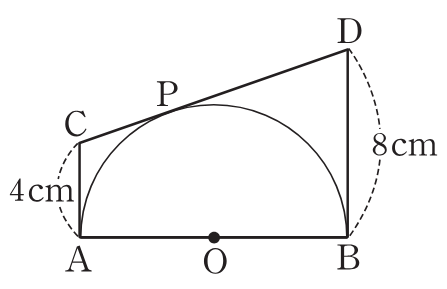
\includegraphics[width=107.2pt]{figures/fig-53-12.png}\end{minipage}\par
\begin{choices32}{\rule[-3ex]{0pt}{8ex}$2\sqrt{21}\mkern3mu \mathrm{cm}$}{\rule[-3ex]{0pt}{8ex}$4\sqrt{6}\mkern3mu \mathrm{cm}$}{\rule[-3ex]{0pt}{8ex}$6\sqrt{13}\mkern3mu \mathrm{cm}$}{\rule[-3ex]{0pt}{8ex}$8\sqrt{2}\mkern3mu \mathrm{cm}$}{\rule[-3ex]{0pt}{8ex}$12\mkern3mu \mathrm{cm}$}\end{choices32}
